\documentclass[runningheads]{llncs}

\usepackage{graphicx}
% \usepackage[english]{babel}
% \usepackage{tikz}
\usepackage{amsmath}
% \usepackage{amsthm}
% \usepackage{listings}
\usepackage{xspace}
% \usepackage{bigstrut}
\usepackage{booktabs}
% \usepackage{subfigure}
% \usepackage{subcaption}
\usepackage{url}
% \usepackage{mathtools}
\usepackage{amsfonts}
\usepackage{amssymb}
\usepackage{multirow}
\usepackage[ruled,vlined]{algorithm2e}
% \usepackage{algpseudocode}
\usepackage{enumitem}
\usepackage{numprint}
% \usepackage[normalem]{ulem}
\usepackage{tcolorbox}
\usepackage{xurl}
\usepackage{xstring}
\usepackage[T1]{fontenc}
\usepackage{pgfplots}
% \usepackage{libertine}
% \usepackage{lmodern}

% % \usepackage{pdflscape}
% \usepackage{rotating}
% \usepackage{caption}
% \usepackage{wrapfig}

\usepackage{color}
% \usepackage[numbers,sort&compress]{natbib}

\usepackage[colorlinks,citecolor=.]{hyperref}
% \urlstyle{tt}
% \hypersetup{
%     colorlinks=true,
%     linkcolor=blue,
%     filecolor=magenta,
%     urlcolor=cyan,
%     pdfpagemode=FullScreen,
% }

% Input Macro File
\definecolor{purple}{rgb}{1, 0, 1}

\newcommand{\ie}{\emph{i.e.,}\xspace}
\newcommand{\eg}{\emph{e.g.,}\xspace}
\newcommand{\abr}{\emph{abbr.}\xspace}
\newcommand{\ea}{\emph{et al.}\xspace}
\newcommand{\gensync}{\emph{GenSync}\xspace}
\newcommand{\colosseum}{\emph{Colosseum}\xspace}
\newcommand{\srep}{\emph{SREP}\xspace} % Set Reconciliation Enhances
\newcommand{\srepsim}{\emph{SREPSim}\xspace}
% Propagation
\newcommand{\esrep}{\emph{E-SREP}\xspace}
\newcommand{\epsrep}{\emph{EP-SREP}\xspace}
\newcommand{\mesrep}{\emph{ME-SREP}\xspace}
\newcommand{\mempoolsync}{\emph{MempoolSync}}

\newcommand{\fref}[1]{Fig.~\ref{#1}}
\newcommand{\tref}[1]{Table~\ref{#1}}
\newcommand{\aref}[1]{Algorithm~\ref{#1}}
\newcommand{\procref}[1]{Procedure~\ref{#1}}
\newcommand{\sref}[1]{Section~\ref{#1}}
\newcommand{\lineref}[1]{line~\ref{#1}}
\newcommand{\appref}[1]{Appendix~\ref{#1}}

% Change \eqref
\LetLtxMacro{\originaleqref}{\eqref}
\renewcommand{\eqref}{Eq.~\originaleqref}

% Theorems and corollaries
\newcounter{theoremcount}
\setcounter{theoremcount}{0}
\DeclareRobustCommand{\theorem}[1]{%
  \refstepcounter{theoremcount}%
  \noindent\textit{\textbf{Theorem \thetheoremcount\label{theorem:#1}: }}%
}
\DeclareRobustCommand{\theoremref}[1]{Theorem~\ref{theorem:#1}}

\DeclareRobustCommand{\proof}{\emph{Proof:}\xspace}
\DeclareRobustCommand{\qqed}{\hfill$\blacksquare$}

\newcounter{corollcount}
\setcounter{corollcount}{0}
\DeclareRobustCommand{\coroll}[1]{%
  \refstepcounter{corollcount}%
  \noindent\textit{\textbf{Corollary \thecorollcount\label{coroll:#1}: }}%
}
\DeclareRobustCommand{\corollref}[1]{Corollary~\ref{coroll:#1}}

\newcounter{lemmacount}
\setcounter{lemmacount}{0}
\DeclareRobustCommand{\lemma}[1]{%
  \refstepcounter{lemmacount}%
  \noindent\textit{\textbf{Lemma \thelemmacount\label{lemma:#1}: }}%
}
\DeclareRobustCommand{\lemmaref}[1]{Lemma~\ref{lemma:#1}}

\newcounter{definitioncount}
\setcounter{definitioncount}{0}
\DeclareRobustCommand{\definition}[1]{%
  \refstepcounter{definitioncount}%
  \noindent\textit{\textbf{Definition \thedefinitioncount\label{definition:#1}: }}%
}
\DeclareRobustCommand{\defref}[1]{Definition~\ref{definition:#1}}

%notes of different authors
\newif\ifnotes
\notestrue
\notesfalse

\newif\ifdiff
\difftrue
\difffalse

\newcommand{\anote}[1]{\ifnotes $\ll$\textsf{\textcolor{purple}{Ari: {#1}}}$\gg$ \fi}
\newcommand{\nnote}[1]{\ifnotes $\ll$\textsf{\textcolor{orange}{Novak: {#1}}}$\gg$ \fi}
\newcommand{\diff}[1]{\ifdiff\textcolor{orange}{#1}\else#1\fi}

%%% Local Variables:
%%% mode: latex
%%% TeX-master: "main"
%%% End:


\newcommand{\etal}{\textit{et al.}\xspace}
\npthousandsep{,}
\npdecimalsign{.}

% \newcommand{\empirical}[1]{{\color{magenta}#1}}
\newcommand{\empirical}[1]{#1}

\newcommand{\block}[1]{\href{https://etherscan.io/block/#1}{#1}\xspace}
\newcommand{\address}[1]{\href{https://etherscan.io/address/#1}{\wrapletters{#1}}\xspace}
\newcommand{\etherscantx}[1]{\href{https://etherscan.io/tx/#1}{\wrapletters{#1}}\xspace}

% wrapping
\newcommand*\wrapletters[1]{\wr@pletters#1\@nil}
\def\wr@pletters#1#2\@nil{#1\allowbreak\if&#2&\else\wr@pletters#2\@nil\fi}

\newcommand{\point}[1]{\par\smallskip\noindent\textbf{#1:}\xspace}
\newcommand{\pointnocolon}[1]{\par\smallskip\noindent\textbf{#1}\xspace}

\newcommand{\protocol}{\textsc{Miqado}\xspace}

\newcommand{\defiMarketSize}{$50$B~USD\xspace}
\newcommand{\defiLendingMarketSize}{$15$B~USD\xspace}
\newcommand{\defiLendingProportion}{$30\%$\xspace}

% %%%%%%%%%%%%%%%%%%%%%%%%%%%%%%%%%%%%%% Empirical Values
\newcommand{\StartDate}{\empirical{1st of May,~2019}\xspace}
\newcommand{\EndDate}{\empirical{30th of September,~2022}\xspace}
\newcommand{\liquidationTimeFrame}{\empirical{$41$~months}\xspace}
\newcommand{\AaveVOneLiquidations}{\empirical{$\numprint{5765}$}\xspace}
\newcommand{\AaveVTwoLiquidations}{\empirical{$\numprint{25576}$}\xspace}
\newcommand{\CompoundLiquidations}{\empirical{$\numprint{17023}$}\xspace}
\newcommand{\TotalLiquidationEvents}{\empirical{$\numprint{48364}$}\xspace}

\newcommand{\LiquidatedCollateral}{\empirical{$\numprint{2.32}$B~USD}\xspace}
\newcommand{\CollateralReleasePeak}{\empirical{$\numprint{653.11}$M~USD}\xspace}
\newcommand{\ShortLiquidations}{\empirical{$\numprint{18305}$}\xspace}
\newcommand{\ShortLiquidationUSDSold}{\empirical{$1.33$B~USD}\xspace}
\newcommand{\FullySoldShortLiquidations}{\empirical{$\numprint{3365}$}\xspace}
\newcommand{\ShortLiquidationsSellPercentageAverage}{\empirical{$95.95\%$}\xspace}
\newcommand{\ShortLiquidationPriceDeclineAverage}{\empirical{$0.38\%$}\xspace}
\newcommand{\ShortLiquidationPriceDeclineMax}{\empirical{$26.90\%$}\xspace}

\newcommand{\CollateralRestraintTwenty}{\empirical{$5.63$B}\xspace}
\newcommand{\CollateralRestraintTen}{\empirical{$2.82$B}\xspace}
\newcommand{\CollateralRestraintFive}{\empirical{$1.41$B}\xspace}
\newcommand{\CollateralRestraintTwo}{\empirical{$563.40$M}\xspace}
\newcommand{\CollateralRestraintOne}{\empirical{$281.70$M}\xspace}

\newcommand{\HealthyPositionsAfterFSL}{\empirical{$82.25\%$}\xspace}
\newcommand{\HealthyPositionsAfterMiqadoLambdaFive}{\empirical{$82.22\%$}\xspace}

\newcommand{\CollateralReleaseWithMiqado}{\empirical{$236.40$M~USD}\xspace}
\newcommand{\CollateralReduction}{\empirical{$89.82\%$}\xspace}



\usepackage{acro}
\acsetup{single}

\DeclareAcronym{DeFi}{
  short = DeFi,
  long  = Decentralized Finance,
}
\newcommand{\DeFi}{\ac{DeFi}\xspace}

\DeclareAcronym{FSL}{
  short = FSL,
  long  = fixed spread liquidation,
}
\newcommand{\FSL}{\ac{FSL}\xspace}

\DeclareAcronym{TVL}{
  short = TVL,
  long  = total value locked,
}
\newcommand{\TVL}{\ac{TVL}\xspace}

\DeclareAcronym{MEV}{
  short = MEV,
  long  = miner extractable value,
}
\newcommand{\MEV}{\ac{MEV}\xspace}

\begin{document}

\title{Mitigating Decentralized Finance Liquidations with Reversible Call Options}
% \title{Introducing Reversible Call Options to Mitigate Decentralized Finance Liquidations}


\author{Kaihua Qin\inst{1}\inst{4} \and
Jens Ernstberger\inst{2}\inst{4} \and
Liyi Zhou\inst{1}\inst{4} \and
 \\ Philipp Jovanovic\inst{3} \and
Arthur Gervais\inst{3}\inst{4}
}
%
\authorrunning{K. Qin et al.}
% First names are abbreviated in the running head.
% If there are more than two authors, 'et al.' is used.
%
% \institute{Imperial College London, United Kingdom\\ \email{\{kaihua.qin,liyi.zhou\}@imperial.ac.uk}\\ \and
% Technical Univeristy Munich, Germany\\ \email{jens.ernstberger@tum.de}\\ \and
% University College London, United Kingdom\\ \email{\{p.jovanovic,a.gervais\}@ucl.ac.uk} }
\institute{Imperial College London, United Kingdom \and
Technical University Munich, Germany \and
University College London, United Kingdom \and
UC Berkeley RDI, United States}

% \author{Kaihua Qin\inst{1} \and
% Jens Ernstberger\inst{3} \and 
% Liyi Zhou\inst{1} \and
% Philipp Jovanovic\inst{2} \and \\
% Arthur Gervais\inst{1}}

% \authorrunning{K. Qin et al.}
% \institute{\instOne, \instTwo, \instThree\\ \email{\{kaihua.qin,liyi.zhou,pablo.gamito17,a.gervais\}@imperial.ac.uk} \and
% University College London, United Kingdom\\ \email{p.jovanovic@ucl.ac.uk}}

\maketitle


\begin{abstract}
Liquidations in \DeFi are both a blessing and a curse~---~whereas liquidations prevent lenders from capital loss, they simultaneously lead to \liquidationSpirals and system-wide failures. Since most lending and borrowing protocols assume liquidations are indispensable, there is an increased interest in alternative constructions that prevent immediate systemic-failure under uncertain circumstances.

In this work, we introduce \textit{\financialPrimitives}, a novel financial primitive that enables the seller of a call option to terminate it before maturity. We apply \financialPrimitives to lending in \DeFi and devise \protocol, a protocol for lending platforms to replace the liquidation mechanisms. To the best of our knowledge, \protocol is the first protocol that actively mitigates liquidations to reduce the risk of liquidation spirals. Instead of selling collateral, \protocol incentivizes external entities, so-called \textit{\supporters}, to top-up a borrowing position and grant the borrower additional time to rescue the debt. Our simulation shows that \protocol reduces the amount of liquidated collateral by~\CollateralReduction in a worst-case scenario.

\keywords{DeFi  \and Liquidation \and Reversible call option.}

%{\color{red}The lending and borrowing markets in \DeFi account with~\defiLendingMarketSize for more than~\defiLendingProportion of the \DeFi's \TVL. Yet, the liquidation mechanisms in \DeFi lending protocols were shown to sell excessive collateral at the borrowers' expenses. 
%Liquidations further harm lending platforms, by reducing the \TVL, which serves as a common success metric of \DeFi platforms.
%Liquidations further trigger downward price spirals of the collateral asset, aggravating the price instabilities of the liquidated collateral. \protocol strengthens blockchain security by reducing the dangers from \MEV.


%We propose \protocol, an add-on protocol for lending platforms mitigating downward price spirals, reducing borrower liquidation losses and increasing lending platforms' \TVL. To the best of our knowledge, \protocol is the first \emph{liquidation prevention protocol}. Instead of selling collateral, the idea is to financially incentivize external entities, so-called \supporters, to top-up any debt position, avoiding liquidations by design and granting borrowers additional time rescuing debt. We provide an empirical evaluation and show how \protocol positively supports the collateral price and .

%We find that liquidations exert a negative pressure on the collateral asset price with an average decline of~\AveravePriceDecrease. We show that \protocol could have instead positively supported the collateral price by an average of~\AveravePriceIncrease, helping to avoid deleveraging collateral price spirals.
%}
\end{abstract}

\acresetall

\section{Introduction}
% Decentralized Finance
Recently, there has been an increasing interest in \DeFi, a financial ecosystem where users exercise cryptographic control over their financial assets.
Commonly, \DeFi is enabled by blockchains that support smart contracts (e.g., Ethereum), and financial primitives are instantiated as publicly accessible decentralized applications. 
A wide variety of traditional financial services that are implemented in \DeFi, ranging from asset exchanges, to market making, as well as lending and borrowing platforms~\cite{qin2021cefi}. 
\DeFi differs from the traditional, centralized financial system in multiple aspects. For instance, most \DeFi services are open-source, such that traders can inspect the protocol rules encoded within immutable smart contracts.% Moreover, all executed transactions are publicly visible, disclosing trading amounts, timestamps and involved assets.

% Lending and borrowing services are important
With over~\defiLendingMarketSize of \TVL, \DeFi's lending and borrowing services account for~\defiLendingProportion of \DeFi's locked up assets. Just as in the traditional centralized finance domain, debt in \DeFi is prone to \emph{liquidation events} upon price-swings of the debts' security deposit (subsequently referred to as collateral). A \borrowingPosition becomes ``unhealthy'' (i.e., liquidatable), whenever the collateral is deemed insufficient to cover the debt, corresponding to a \emph{health factor} inferior to one. The most prevalent liquidation mechanism, \FSL, allows a \emph{liquidator} to repay a fraction  of the borrower's debt and acquire its collateral at a discount. The fraction at which the borrowers' debt is repaid in a liquidation is limited to an upper bound, commonly referred to as the \emph{close factor} (e.g.,~\href{https://docs.aave.com/developers/v/2.0/guides/liquidations#0.-prerequisites}{$50\%$}). 
As such, liquidations intend to protect the lender by preventing a loss of capital by selling a sufficient amount of collateral.
However, liquidations serve as a double-edged sword. Selling off collateral causes a price decrease, which potentially leads to further liquidations and market-wide panic~\cite{klages2019stability}.
Quantifying the extent of liquidations in \DeFi, a recent two-year longitudinal study (April $2019$ to April $2021$) by Qin \emph{et al.}~\cite{qin2021empirical} finds that liquidation events on the Ethereum blockchain amount to over $800$M USD in volume, yielding a staggering $64$M USD profit to liquidators. Such liquidation profit constitutes a source of \MEV~\cite{daian2020flash}, which grants miners a risk-free opportunity to extract financial profit. \MEV, however, negatively affects blockchain consensus security by incentivizing blockchain forks~\cite{qin2022quantifying}.
%Liquidations moreover result in \textit{liquidation spirals}, where the price decline resulting from sold-off collateral results in a price drop that triggers further liquidations.



%\subsubsection{Miner Extractable Value (MEV)} Daian \etal~\cite{daian2020flash} propose the concept of miner extractable value. In a blockchain system, a miner has the authority to determine the transaction execution order within a mined block, which provides the miner with advantages in competing for a profitable opportunity (e.g., liquidations). A miner is able to execute its own value extracting transaction first (i.e., by front-running all competitors) when detecting such trading opportunity. These risk-free value extractions through transaction order manipulation are referred to as MEV. MEV has been shown to be a significant blockchain consensus security problem~\cite{daian2020flash,zhou2021just,qin2022quantifying}, because miners might deliberately fork a blockchain to compete for a profitable opportunity. Qin \etal~\cite{qin2021empirical} show that existing fixed spread liquidations contribute significantly to MEV. However, in \protocol, due to the unpredictability of currency prices, miners cannot extract risk-free value through tolling, though they maintain an advantage in front-running other tollers for the \protocol initiation.

In this work, we propose \protocol, a mechanism designed to mitigate liquidation events to \textit{(i)}~protect borrowers from excessive collateral liquidation, \textit{(ii)}~alleviate \MEV sourcing, and \textit{(iii)}~mitigate \liquidationSpirals. 
%\protocol allows third parties to support the borrower in rescuing debt which is close to being liquidated.
%The secret sauce of \protocol is to allow third parties to participate in rescuing debt which may be on the brink of being liquidated.
To this end, we introduce \textit{\financialPrimitives}, a novel financial primitive that enables the seller of a call option to terminate it at a premium before reaching maturity.
\protocol applies \financialPrimitives to incentivize external support for ``unhealthy'' borrowing positions, while the original borrower is granted additional time to protect its borrowing position and limit the potential loss. 
%As a by-product, \protocol also increases the lending platforms' \TVL, which is a common protocol success metric.
% \protocol adds a risk component that negatively impacts \MEV extraction from liquidation events, and hence disincentivizes \MEV while improving blockchain consensus security.

Thereby, we summarize the contributions of this work as follows.
\begin{enumerate}
    \item \textbf{Quantifying \LiquidationSpiral.} We quantify the \liquidationSpiral caused by the \FSL mechanism by analyzing~\TotalLiquidationEvents past liquidation events over a time-frame of~\liquidationTimeFrame, capturing~\LiquidatedCollateral of collateral liquidated. We find the existence of~\ShortLiquidations short liquidations, where a liquidator immediately sells the acquired collateral.
    %where a liquidator sells the acquired collateral within the liquidation transaction. 
    These liquidations account for~\ShortLiquidationUSDSold sold collateral and a maximal collateral price decline of~\ShortLiquidationPriceDeclineMax.
    %~\ShortLiquidationUSDSold of collateral is sold in these short liquidations, causing a collateral price decline of~\ShortLiquidationPriceDeclineAverage on average.
    %\item \textbf{\protocol evaluation.} We empirically simulate how \protocol would have performed in the past liquidation events. Our results show that \protocol reduces the amount of liquidated collateral by~\CollateralReduction in a worst-case scenario.
    % Financial Primitive
    \item \textbf{A Novel Financial Primitive.}
    We introduce \financialPrimitives, a novel financial primitive where the seller of a European call option can pay a premium to the buyer to terminate the option before its maturity.
    % Liquidation Mitigation
    \item \textbf{A Protocol for Liquidation Mitigation.} We propose \protocol, the first protocol that protects \DeFi borrowers from excessive liquidation losses. 
    By realizing a \financialPrimitive, \protocol incentivizes external actors to support ``unhealthy'' \borrowingPositions, mitigating liquidations by design. 
    %Leveraging the \financialPrimitive, a novel \DeFi primitive introduced in this work, \protocol incentivizes external actors to support ``unhealthy'' \borrowingPositions, mitigating liquidations by design. 
    %\item \textbf{Plug \& Play Liquidation Mitigation Mechanism.} To the best of our knowledge, we are the first to devise a permissionless algorithm to protect \DeFi borrowers from excessive liquidation losses. Leveraging the \financialPrimitive, a novel \DeFi primitive introduced in this work, \protocol incentivizes external actors to support ``unhealthy'' \borrowingPositions, mitigating liquidations by design. 
    \protocol serves as a plug-and-play mechanism, which can be integrated into any existing lending platform. 
    We evaluate \protocol by simulating how it would have performed in past liquidation events. We find that \protocol reduces the amount of liquidated collateral by~\CollateralReduction in a worst-case scenario.
    %Further, we show that applying the \protocol protocol guarantees an increased \borrowingPosition health factor, which cannot be guaranteed by existing liquidation mechanisms.
\end{enumerate}

%\begin{description}[style=unboxed, leftmargin=0cm]
%\item[Plug \& Play Liquidation Mitigation Mechanism] To the best of our knowledge, we are the first to devise a permissionless algorithm to protect \DeFi borrowers from excessive liquidation losses. \protocol incentivizes external actors to rescue debt positions, preventing liquidations by design. \protocol serves is a plug-and-play mechanism, which can be integrated into any existing lending platform.
%We show that \protocol guarantees an increased \borrowingPosition health factor, which cannot be guaranteed by existing liquidation mechanisms. %\protocol serves as a plug-and-play mechanism for existing lending protocols.
%which can be adopted in e.g., Aave, one of the biggest \DeFi lending platforms, by simply replacing the lending manager contracts.
%e.g., by simply replacing the lending manager contracts in Aave, one of the biggest lending platforms at the time of writing.
%\item[Quantifying Downward Price Spiral] We quantify the downward price spiral caused by the \FSL mechanism by analyzing~\TotalLiquidationEvents past liquidation events over a time-frame of~\liquidationTimeFrame, capturing~\LiquidatedCollateral of collateral liquidated. We find the existence of~\ShortLiquidations pessimistic short, where a liquidator sells the acquired collateral within the liquidation transaction.~\ShortLiquidationUSDSold of collateral is sold in these pessimistic liquidations, causing a collateral price decline of~\PessimisticLiquidationPriceDeclineAverage on average.

% \item[MEV Deterrence:] \protocol does not prevent, but mitigates liquidation MEV by adding a risk component to a previously risk-free MEV opportunity. Increasing the risks of MEV sourcing deters its extraction and hence contributes to blockchain consensus security.
%\item[\protocol Evaluation] We empirically evaluate \protocol by simulating how \protocol could have performed in the xxx past liquidation events. We find that ....

%We evaluate \protocol empirically through simulations and empirical comparisons to a total of~\StudiedLiquidations past liquidation events. We detect~\LiquidationsMayNineteen liquidations on the 19th of May 2021, when the cryptocurrency market declined by an average of $40$\%. If \protocol had been widely adopted, the studied lending platforms Aave and Compound could have absorbed an additional~\TotalDepositedCollateral of collateral (a plus of~$5.24\%$), instead of losing~\TotalBorrowerLoss in TVL (a loss of~$0.15$\%) within a single day. Similarly, for the~21st of May/the~7th of September,~2021, lending pools could have attracted~\TotalDepositedCollateralMayTwentyFirst/\TotalDepositedCollateralSept of collateral with \protocol, instead of losing~\TotalLostCollateralMayTwentyFirst/\TotalLostCollateralSept of TVL through~\LiquidationsMayTwentyFirst/\LiquidationsSept liquidations.

% \item[Mitigating Deleveraging Spiral:] We show that liquidations negatively impact the collateral price, which may result in further liquidations. We show that these liquidations affect the on-chain collateral price by~\AveravePriceDecrease on average. By avoiding liquidations, \protocol could have supported the average collateral price by~\AveravePriceIncrease.
%\end{description}


\section{Background}\label{sec:background}
% In this section, we outline the required background of blockchains and decentralized finance (DeFi) ecosystems.

\subsection{Blockchain \& Smart Contract}
In essence, a blockchain is a distributed ledger operating on top of a peer-to-peer (P2P) network~\cite{bonneau2015sok}. The core blockchain functionality is that participants can transfer financial assets (i.e., cryptocurrencies) without any trusted third-party custodian~\cite{bitcoin}. To send cryptocurrencies, one broadcasts a signed transaction through the blockchain P2P network. The so-called \emph{miners} collect, verify and package transactions into a block which is appended onto the already confirmed blocks forming a linear chain. All peers in the blockchain network are expected to follow a specific consensus mechanism (e.g., Nakamoto consensus~\cite{bitcoin}) to achieve the consistency of the ledger.

Beyond the simple cryptocurrency transfer, more versatile blockchains (e.g., Ethereum~\cite{wood2014ethereum}) enable advanced transaction logic through pseudo-Turing complete smart contracts. Similar to regular user accounts, smart contracts can own cryptocurrencies. In addition, every smart contract is bound to a piece of immutable code upon its creation. Users can send a transaction to a smart contract account and trigger the execution of the associated smart contract code. We refer readers to~\cite{bonneau2015sok} for more detailed explanations of blockchains and smart contracts.

\subsection{Decentralized Finance}
Smart contracts enable the creation of cryptocurrencies (also known as tokens) on a blockchain in addition to the native cryptocurrency (e.g., ETH on Ethereum). A token smart contract serves as a balance sheet recording the balance of every token holder account. Smart contracts also allow anyone to create any type of imaginable financial product on-chain, by enforcing the rules through the smart contracts' immutable code. The ecosystem as a whole, composed of these tokens and smart contract-based financial products, is referred to as \DeFi. At the time of writing, the scale of \DeFi has reached over~\defiMarketSize, with an abundance of applications such as exchanges, lending platforms, and derivatives.\footnote{\url{https://defillama.com/}.}

\subsection{Lending/Borrowing in \DeFi}\label{sec:background-lending-borrowing}
Lending and borrowing, with over~\defiLendingMarketSize \TVL, is one of the most popular \DeFi use cases. In a \DeFi lending system, a smart contract called \emph{lending pool}, manages the \borrowingPositions.
% Lenders can provide assets for borrowing by depositing cryptocurrencies into the lending pool, while borrowers borrow cryptocurrencies from the pool.
Lenders provide assets to the lending pool to earn interests from borrowers. To minimize the lenders' risk of losing funds, every borrower is required to provide \emph{collateral} as a guarantee.
The lending and borrowing interests are programmatically determined by the contract code.

Lending in \DeFi can be divided into \emph{over-collateralized} and \emph{under-collateralized} lending. In over-collateralized lending, the borrower provides a security deposit (i.e., collateral) which \emph{exceeds} the lent assets by a factor of $1.1\times$ to $2\times$ depending on the respective protocol~\cite{qin2021empirical}. The borrower may then choose to freely use the lent asset in any capacity. Contrary to over-collateralized lending, in under-collateralized lending, the borrower only provides a fraction of the lent assets as security, hence achieving a leverage factor beyond $1\times$. For this leveraged borrowing to remain secure, the assets granted through under-collateralization can only be utilized in very specific, hard-coded settings encoded in immutable smart contracts, such that the lending pools stay in control of the lent assets. In this work, we primarily focus on over-collateralized lending.

We refer to the debts of a borrower together with the collateral securing these debts as a \emph{borrowing position}. Due to asset price fluctuations, the collateral of a borrowing position may become insufficient to cover the debt. Therefore, lending pools typically set a threshold for the borrowing positions, at which a position becomes liquidatable. When the collateral value of a borrowing position declines below this threshold, lending pools can then allow the so-called liquidators, to repay the debt for the position, commonly referred to as liquidation. In return, the liquidator is eligible to acquire parts of the collateral from the borrowing position. The acquired collateral exceeds the repaid debt in value, which incentivizes the liquidator to realize a profit.

% \paragraph{Price Oracles}
% Lending pools are required to have access to the real-time cryptocurrency prices in order to estimate the collateral and debt value. To report such prices, price oracles~\cite{liu2021first,eskandari2021sok} feed smart contracts with the desired asset prices. On a high level, at the time of writing there exist three oracle mechanisms: \textit{(i)}~off-chain price sources (e.g., centralized exchanges) update the price oracles periodically; \textit{(ii)}~on-chain exchanges can be requested to act as price oracles; \textit{(iii)}~a combination of the two aforementioned mechanisms.

% \begin{table}[t]
%     \centering
%     \renewcommand{\arraystretch}{1.1}
%     \caption{Notation.}
%     \resizebox{0.8\textwidth}{!}{%
%     \begin{tabular}{rcl c rcl}
%     \toprule
%     \multicolumn{1}{r}{\bf Symbol} & \phantom{a} & \multicolumn{1}{l}{\bf Description} & \phantom{aaaa} & 
%     \multicolumn{1}{r}{\bf Symbol} & \phantom{a} & \multicolumn{1}{l}{\bf Description} \\
%     \cmidrule(rl){1-3}\cmidrule(rl){5-7}
%      %$\mathcal{L}$ && Lending pool && $\collateralDiscountShort$ && Collateral discount \\
%      $\cryptocurrencyDebt$ && Debt Cryptocurrency && $\numberCoinsDebt$ && \# Coins Debt \\
%      $\cryptocurrencyCollateral$ && Collateral Cryptocurrency && $\numberCoinsCollateral$ && \# Coins Collateral \\
%      $\borrowerShort$ && \Borrower && $\healthFactorShort{\borrowingPositionShort{}}$ && \HealthFactor \\
%      $\lenderShort$ && \Lender && $\closeFactorShort$ && \CloseFactor \\
%      $\supporterShort$ && \Supporter && $\collateralizationRatioShort{\borrowingPositionShort{}}$ && \CollateralizationRatio \\
%      $\liquidatorShort$ && \Liquidator && $\liquidationSpreadShort$ && \LiquidationSpread \\
%      $\lendingPoolShort$ && \LendingPool && $\collateralDiscountShort$ && \CollateralDiscount \\
%      $\borrowingPositionShort{}$ && \BorrowingPosition &&  &&  \\
     
%     \bottomrule
%     \end{tabular}%
%     }
%     \label{tab:notations}
% \end{table}

\subsection{Call Options}\label{section:callOption}
Call options are financial contracts that grant buyers the right, but not the obligation, to buy an underlying asset (e.g., stocks) at an agreed-upon price (i.e., the exercise price or strike price) and date (i.e., the expiration date or maturity)~\cite{stoll1969relationship,hull2003options}. 
In general, options are priced using a mathematical model, such as the Black-Scholes~\cite{black1973pricing} or the Binomial pricing model~\cite{shreve2005stochastic}.
On a high level, an options price is determined by \emph{(i)} its intrinsic value and \emph{(ii)} its time value.
The intrinsic value is a measure of the profitability of an option if it were to be exercised immediately.
The time value measures the value of an option arising from the time left to maturity (i.e., volatility).
When the strike price of an option increases, the price of the call option consequently increases as well.
In traditional finance, there are two styles of option contracts: \textit{(i)} American options can be executed (or exercised) at any time up to the expiration date; \textit{(ii)} European options can be exercised only on the expiration date~\cite{hull2003options}. 

% \section{Modeling Lending \& Borrowing Mechanisms}\label{sec:preliminaries}
\section{Preliminaries}\label{sec:preliminaries}

In the following, we formalize a collateralized debt model and the fixed spread liquidation, which is the prevalent \DeFi liquidation mechanism.

\subsection{Collateralized Debt Model}\label{sec:collateralized-debt-model}
%We start by extending the lending system model of Section~\ref{sec:borrowingandlendingsystemmodel}.

% Lending Pool
We assume the existence of an on-chain lending pool $\lendingPoolShort = \{\borrowingPositionShort{1}, \borrowingPositionShort{2}, ..., \borrowingPositionShort{n}\}$, where $\borrowingPositionShort{i}$ is the $i$-th \borrowingPosition in the lending pool.
% Borrowing Position
Each \borrowingPosition $\borrowingPositionShort{} = \langle \numberCoinsDebt{t}, \numberCoinsCollateral{t} \rangle$ is parametrized by the debt $\numberCoinsDebt{t}$ the borrower owes, and the collateral $\numberCoinsCollateral{t}$ the borrower owns at time $t$.
% Price
We denote the price of the debt cryptocurrency towards the collateral cryptocurrency, provided by an oracle~\cite{eskandari2021sok}, as $\price$.
% Monetary Value
% We consider: Simple case, one currency for debt, one for collateral.
In the following, we consider the case where each \borrowingPosition consists of a single debt cryptocurrency and a single collateral cryptocurrency.
In practice, a \lendingPool may allow for mixed \borrowingPositions by including multiple cryptocurrencies as either debt or collateral.
We further assume that a borrower only opens a single \borrowingPosition.

% Health Factor / Parameters for a position
% Each position is defined by...
Whether or not a \borrowingPosition is \textit{liquidatable} is determined by the \textit{\healthFactor}.
\begin{equation}\label{eq:hft}
    \healthFactorShort{\borrowingPositionShort{}}=\frac{\numberCoinsCollateral{t} \cdot \price \cdot \collateralDiscountShort}{\numberCoinsDebt{t}}
\end{equation}
$\numberCoinsCollateral{t} \cdot \price$ represents the value of the collateral, whereas $\numberCoinsDebt{t}$ represents the value of the debt denoted in the same cryptocurrency. $\collateralDiscountShort$ is the collateral discount, s.t. $0 < \collateralDiscountShort < 1$. The \collateralDiscount is configured as a safety margin to ensure the over-collateralization of a position, i.e., the value of the collateral is discounted when calculating the health factor. If $\healthFactorShort{\borrowingPositionShort{}} < 1$, e.g., due to price fluctuations, $\borrowingPositionShort{}$ is deemed ``unhealthy'' making it available for liquidations under existing prevalent designs of \DeFi lending protocols.
% Collateralization Ratio
Internally, the \healthFactor of a \borrowingPosition relies on the \textit{\collateralizationRatio}

\begin{equation}\label{eq:cr}
    \collateralizationRatioShort{\borrowingPositionShort{}}=\frac{\numberCoinsCollateral{t} \cdot \price}{\numberCoinsDebt{t}}.
\end{equation}
The \collateralizationRatio determines whether a position is over-collateralized or under-collateralized. 
If $\collateralizationRatioShort{\borrowingPositionShort{}} > 1$ at time $t$, a position is over-collateralized, and under-collateralized otherwise.


\subsection{Fixed Spread Liquidation}\label{sec:fixed-spread-liquidation}

% Fixed Spread Liquidation Model
We denote a decentralized application for lending and borrowing that applies a fixed spread liquidation mechanism as protocol $\fixedSpreadProtocol$. For ease of exposition, we assume that $\fixedSpreadProtocol$ hosts a single lending pool $\lendingPoolShort$. 
% Parametrized by the collateral discount, the close factor as well as the liquidation spread
The liquidation of a position $\borrowingPositionShort{} = \langle \numberCoinsDebt{t}, \numberCoinsCollateral{t} \rangle$  is determined by a set of variables, %which determine the amount of collateral $\numberCoinsCollateral{t}' \leq \numberCoinsCollateral{t}$ that can be liquidated once a position is liquidatable.
% Discount = Safety margin 
% Spread = Bonus that liquidator can obtain 
including the previously introduced \collateralDiscount $\collateralDiscountShort$, the \closeFactor $\closeFactorShort$ (s.t.\ $0<\closeFactorShort\leq1$) and the  \liquidationSpread $\liquidationSpreadShort$.

\begin{equation}\label{eq:fsl}
    \fixedSpreadProtocol = \langle \lendingPoolShort, \collateralDiscountShort, \closeFactorShort, \liquidationSpreadShort \rangle
\end{equation}

The \closeFactor $\closeFactorShort$ describes the percentage of debt that the liquidator can repay in a single fixed spread liquidation.
The spread $\liquidationSpreadShort$ is the discount at which the liquidator can obtain the collateral. $\liquidationSpreadShort$ is fixed throughout the execution of the protocol (i.e., the name \textit{fixed spread liquidation}).
With the liquidation spread, one can calculate the maximal collateral claimable by the liquidator $\liquidatorShort$ as $(\numberCoinsDebt{t} \cdot \closeFactorShort) \cdot (1+\liquidationSpreadShort)$. 
Without consideration of gas fees, the maximal obtainable profit by $\liquidatorShort$ is $(\numberCoinsDebt{t} \cdot \closeFactorShort) \cdot \liquidationSpreadShort$.
As the protocol is overall a zero-sum game, and under the assumption of non-existant slippage, the profit of the \liquidator is equivalent to the borrowers loss, if denoted in the same cryptocurrency.

Other liquidation mechanisms, though operated differently from the fixed spread liquidations, follow similar high-level designs --- debts are repaid in exchange for collateral from the liquidated borrowing position. For example, in MakerDAO auction liquidations, liquidators bid for the liquidation opportunity by submitting transactions~\cite{qin2021empirical}. In such a setting, the liquidation spread can hence be considered dynamic during the auction execution.






% \subsection{OLD Collateralized Debt Model}
% We assume the existence of an on-chain lending pool $\mathcal{L} = \langle \mathcal{C}, \mathcal{D}, \mathcal{P}\rangle$, where $\mathcal{C}=\{C_1, C_2, ..., C_n\}$ denotes the set of collateral cryptocurrencies; $\mathcal{D} = \{D_1, D_2, ..., D_n\}$ denotes the set of debt cryptocurrencies available for borrowing; $\mathcal{P}=\{P_1, P_2, ..., P_n\}$ denotes the set of borrowing positions. In practice, a borrowing position may be opened with multiple collateral and debt cryptocurrencies. To ease understanding, in our analytical model, we only consider a single collateral cryptocurrency, denoted by $C$, and a single debt cryptocurrency, denoted by $D$. By collateralizing into and then borrowing from $\mathcal{L}$, a borrower $\mathcal{B}$ is allowed to open a borrowing position $P = \langle C, D\rangle$, where $C\in\mathcal{C}$ denotes the collateralized cryptocurrency, while $D\in\mathcal{D}$ denotes the borrowed cryptocurrency. We assume that every borrower only opens one borrowing position in $\mathcal{L}$. Hence, in the following, $P_\mathcal{B}$ denotes the borrowing position of a borrower $\mathcal{B}$.

% We define $\mathsf{Collateral}_t(P_\mathcal{B})$ and $\mathsf{Debt}_t(P_\mathcal{B})$ to represent the amount of collateral and debt that a borrower $\mathcal{B}$ owns and owes respectively in $\mathcal{L}$ at time $t$. We denominate the monetary value of the collateral and debt with $D$. The price of $C$ with respect to $D$ at time $t$ published by an oracle (cf.\ Section~\ref{sec:background-lending-borrowing}) is denoted by $p_t$. In practice, the time in a DeFi ecosystem is typically measured in the number of blocks or follows the block timestamps. $\mathcal{L}$ is required to monitor and maintain the health of every borrowing position. The health factor function of a borrowing position $P_\mathcal{B}$ is formulated in Equation~\ref{eq:hft}.

% \begin{equation}\label{eq:hft}
%     \mathsf{HF}_{t}(P_\mathcal{B})=\frac{\mathsf{Collateral}_t(P_\mathcal{B})\cdot p_t\cdot\mathbf{CD}}{\mathsf{Debt}_t(P_\mathcal{B})}
% \end{equation}
% $\mathsf{Collateral}_t(P_\mathcal{B})\cdot p_t$ represents the value of the collateral while $\mathsf{Debt}_t(P_\mathcal{B})$ represents the value of the debt. $\mathbf{CD}$ is the collateral discount, s.t. $0 < \mathbf{CD} < 1$. $\mathbf{CD}$ is configured to leave a safety margin ensuring the over-collateralization of a position, i.e., the value of the collateral is discounted when calculating the health factor. If $\mathsf{HF}_t(P_\mathcal{B}) < 1$, e.g., due to price fluctuations, $P_\mathcal{B}$ is deemed ``unhealthy'' making it available for liquidations under existing prevalent designs of DeFi lending protocols. We proceed to define the collateralization ratio of a borrowing position $P_\mathcal{B}$ as the ratio between the value of the collateral and the debt (cf.\ Equation~\ref{eq:cr}). We consider $P_\mathcal{B}$ to be over-collateralized, when $\mathsf{CR}_t(P_\mathcal{B})>1$, and under-collateralized otherwise.
% \begin{equation}\label{eq:cr}
%     \mathsf{CR}_t(P_\mathcal{B})=\frac{\mathsf{Collateral}_t(P_\mathcal{B})\cdot p_t}{\mathsf{Debt}_t(P_\mathcal{B})}
% \end{equation}

% \subsection{OLD Fixed Spread Liquidation}

% A fixed spread liquidation protocol is parameterized by the collateral discount $\mathbf{CD}$ (cf.\ Section~\ref{sec:collateralized-debt-model}), the close factor $\mathbf{CF}$, and the liquidation spread $\mathbf{LS}$.

% \begin{equation}\label{eq:fixed-spread-liquidation}
% \pi_\text{FL} = \langle \mathcal{L}, \mathbf{CD}, \mathbf{CF}, \mathbf{LS} \rangle
% \end{equation}
% The close factor limits the single liquidation size, while the liquidation spread specifies the rewards that the liquidator receives.
% Specifically, to liquidate a borrowing position $P_\mathcal{B}$, a liquidator $\mathcal{Q}$ repays $d$ amount of $D$ for $P_\mathcal{B}$ at time $t$. The amount $d$ is constrained by $\mathbf{CF}$, s.t.\ $d\leq\mathbf{CF}\cdot\mathsf{Debt}_t(P_\mathcal{B})$. In return, $\mathcal{Q}$ is allowed to acquire $\frac{d(1+\mathbf{LS})}{p_t}$ amount of collateral $C$ from $P_\mathcal{B}$. Hence $\mathcal{Q}$ realizes a profit of $d\cdot\mathbf{LS}$ (denominated in $D$). Note that for simplicity we ignore the transaction fees required by the underlying blockchain.

% Other liquidation mechanisms, though operated differently from the fixed spread liquidations, follow similar high-level designs --- debts are repaid in exchange for collateral from the liquidated borrowing position. For example, in MakerDAO auction liquidations, liquidators bid for the liquidation opportunity by submitting transactions~\cite{qin2021empirical}. In such a setting, the liquidation spread can hence be considered dynamic during the auction execution.

% % we assume that the health factor of $P_\mathcal{B}$ declines below $1$ at time $t$. $\mathcal{Q}$ then repays $x$ amount of $D$ for $P_\mathcal{B}$. $x$ is constrained by the close factor $\mathbf{CF}$, s.t. $x \leq \mathbf{CF}\cdot\mathsf{Debt}_t(P_\mathcal{B})$. In $y = \frac{z}{p_t}(1+\mathbf{LS})$.

% % 
% }


% % Such collateral selling behaviors are impossible in the \protocol protocol, because the collateral is locked in the lending pool until \protocol terminates. Moreover, the toller needs to purchase collateral from other markets, if the toller does not hold any cryptocurrency collateral to initiate \protocol. This purchase may help suppress the downtrend of the collateral price. Given the studied liquidation, if Compound were to adopt the \protocol protocol, the toller would be required to collateralize $\numprint{4092.60}$ ETH\footnote{At the time of the liquidation, the borrowing position held $\numprint[ETH]{12277.80}$ of collateral and the collateral discount of ETH is $0.75$. Hence, in \protocol, the ETH required to be collateralized can be calculated from $(\frac{1}{0.75}-1)\times\numprint{12277.80}=\numprint[ETH]{4092.60}$.} into lending pool. We further assume that the toller purchases the required ETH from the same Uniswap USDC/ETH market before initiating \protocol, which requires the sale of $11.0$M USDC. The ETH price then immediately increases from~$\numprint{2477.96}$ USDC/ETH to~$\numprint{2912.00}$ USDC/ETH ($+17.52\%$). It is worth noting that at the time of the studied liquidation, to the best of our knowledge, Uniswap was the deepest USDC/ETH market on Ethereum, which provided a liquidity of $52.68$K ETH and $130.53$M USDC. We remark that a significant price change in a single market will eventually be evened out by arbitrageurs\footnote{Entities who profit by leveraging price differences across different markets.} among all available markets, while the negative impact on the collateral price remains.%However, our case study is sufficient to indicate the impact of liquidations and \protocol on the collateral price.
% % We repeat our case study on two further liquidations\footnote{Tx hashes: \etherscantx{0xa4fbc05b794aa987b8f118680da67f157cc65821f49b10403e7a0b19b0d14e0b} and \etherscantx{0x5ea812c62ccbe9527ef4317b97aa220e50c16d51844a8940ee31c01a11dd7556}.}. We find that these two liquidations decrease the collateral price by~$4.73\%$ and $6.62\%$, while \protocol could have increased the collateral price by $29.30\%$ and $4.78\%$ respectively.

% % Out of a total of~\StudiedLiquidations investigated liquidation events, we find that the collateral of~\PriceChangeLiquidations liquidations is sold in the same transaction. On average, the subsequent exchange decreases the collateral price in the corresponding on-chain market by~\AveravePriceDecrease, while \protocol could have increased the price by~\AveravePriceIncrease. A high price increase implies a substantial slippage (traders transact at a worse price than the market price due to insufficient liquidity~\cite{zhou2020high}) when a toller purchases collateral. This slippage cost may discourage potential tollers from engaging in \protocol, which is further discussed in Appendix~\ref{app:extended-analysis}.

\section{Motivation}\label{sec:motivation}
We proceed to outline the design flaws of liquidation mechanisms and motivate why mitigating liquidations is necessary.

\begin{enumerate}
    \item \textbf{Over-Liquidation.} \DeFi borrowers are exposed to an unnecessarily overwhelming liquidation risk. In regular \FSL configurations,~$50\%\sim 100\%$ of a borrowing position is liquidated within a single transaction~\cite{qin2021empirical,wang2022speculative}.

    \item \textbf{\MEV.} Liquidation is one of the major sources of \MEV, which disrupts miner incentives and endangers the consensus security of a blockchain~\cite{qin2022quantifying}.
    
    \item \textbf{\LiquidationSpiral.} A liquidation increases the supply of the collateral cryptocurrencies available for sale. This supply inflation imposes a negative impact on the collateral prices~\cite{whelan2001economic} and may result in further liquidations (possibly \liquidationSpiral~\cite{klages2019stability}). We provide a case study of a real liquidation event to present the impact of liquidations on collateral prices.
\end{enumerate}

% \begin{description}
% \item[Over-Liquidation] Under regular configurations of \FSL,~$50\%\sim 100\%$ of a borrowing position might be liquidated within a single transaction upon a price decline~\cite{qin2021empirical,wang2022speculative}. \DeFi borrowers are hence exposed to an unnecessarily overwhelming liquidation risk.
% \item[\MEV] Liquidation is one of the major sources of \MEV, which disrupts miner incentives and endangers the consensus security of a blockchain~\cite{qin2022quantifying}.
% \item[Deleveraging Spiral] A liquidation increases the supply of the collateral cryptocurrencies available for sale. This supply inflation imposes a negative impact on the collateral prices~\cite{whelan2001economic} and may result in further (possibly deleveraging spiral~\cite{klages2019stability}) liquidations. We provide a case study of a real liquidation event to present the impact of liquidations on collateral prices.
% %A liquidation decreases the supply of the debt cryptocurrencies in the market, while making further collateral available for sale. Following the relations among supply, demand and price~\cite{whelan2001economic}, liquidations impose a negative impact on the collateral prices and may result in further (possibly deleveraging spiral~\cite{klages2019stability}) liquidations.
% \end{description}

% We proceed to provide a case study of a real liquidation event to present the impact of liquidations on collateral prices.

\begin{figure}[h]
    \centering
    \includegraphics[width=\columnwidth]{figures/liquidation_case_study.pdf}
    \caption{A real liquidation event with a subsequent downward price trend of the collateral asset. The liquidator $\liquidatorShort$ immediately sold parts of the redeemed ETH collateral from a Compound liquidation, which decreased the ETH price on Uniswap by $6.95\%$.}
    \label{fig:liquidation-case-study}
\end{figure}

\newtheorem{casestudy}{Case Study}
\begin{casestudy}[\LiquidationSpiral]\label{casestudy:deleveraging-spiral}
As shown in Figure~\ref{fig:liquidation-case-study}, two \DeFi platforms were involved in this liquidation: (i) Compound, an over-collateralized lending platform; (ii) Uniswap, an on-chain exchange. USDC is a stablecoin, of which the value is pegged to USD.\footnote{Transaction hash: \etherscantx{0xe7b6fac6502be7c6659880ff5d342ec470429c6f49cd457945bf0726667eb689}. Note that we ignore the irrelevant execution details to ease understanding.}  In the studied liquidation, the liquidator mainly took the following three steps.

\begin{enumerate}
    \item The liquidator repaid~$4.61$M USDC for a Compound borrowing position.
    \item In return, the liquidator was allowed to redeem $\numprint{2034.64}$ ETH of collateral.
    \item The liquidator bought $\numprint{1933.43}$ ETH from the redeemed collateral and exchanged the ETH for $4.61$M~USDC to cover its repayment cost in Step 1. The liquidator realized a profit of~$101.20$ ETH through this liquidation.
\end{enumerate}
In the third step, the exchange from ETH to USDC on Uniswap USDC/ETH triggered a price decline from~$\numprint{2477.96}$ USDC/ETH to~$\numprint{2305.85}$ USDC/ETH ($-6.95\%$). This event shows that even a single liquidation can decrease the collateral price significantly.
\end{casestudy}

\subsubsection{Why collateralization instead of liquidation?}
In this work, \protocol requires additional collateral to be locked in the lending pool, reducing the liquid collateral asset supply. Hence, we conclude that \protocol behaves more positively than a liquidation mechanism on stabilizing lending markets, effectively acting like a price ``softening buffer''. We empirically confirm this effect in Section~\ref{sec:empirical}.


\section{\protocol}\label{sec:toll}
% \point{Design Requirement}
% \begin{itemize}
%     \item Incentivize borrowers to top up collateral or repay debt as soon as possible.
%     \item Incentivize tollers to collateralize for the unhealthy borrowers.
%     \item Attract more collateral for the lending pool.
% \end{itemize}
% {\color{blue}
% In this section, we present \protocol, which is a mechanism designed to secure collateralized debts and mitigate the utilization of liquidations. To this end, we introduce a new actor called toller. Given an unhealthy borrowing position, instead of repaying debt and acquiring collateral, a toller deposits additional collateral into the position. 
% }


In this section, we introduce \protocol. \protocol is a debt management mechanism for \DeFi lending protocols. 
It mitigates liquidations through a set of incentives that decrease the likelihood of \liquidationSpirals.  
\protocol relies on \textit{\supporters}, which are entities that are willing to top up unhealthy borrowing positions. To enable \protocol, we introduce \textit{\financialPrimitives}, a novel financial primitive where the seller of a call option can pay a premium to terminate the contract before maturity.
% To facilitate the \protocol protocol, we introduce a novel financial primitive, which we call \textit{\financialPrimitive}.
% A \financialPrimitive is a traditional call option, with the additional opportunity for the entity handing out the call option to cancel the contract by paying the taker of the call option a premium.
% In the following, we first introduce the \financialPrimitive, and successively show it's application in \protocol.

\subsection{\FinancialPrimitive}


% Recall Call Option from 3.3
Recall the notion of European call options as introduced in Section~\ref{section:callOption}.
In a European call option, the seller offers the option contract whereas the buyer acquires the option to exercise the right to buy an asset at a specific price by buying said option at a premium (i.e., the option price).
The outcome of a European call option contract at maturity is binary~---~\emph{(i)} the buyer exercises its right to buy or \emph{(ii)} the buyer does not exercise its right to buy.
We now introduce the \textit{reversible} European call option, which augments the traditional European call option with an additional outcome to the option contract, where the seller is able to terminate the contract at a premium. 

We say that a reversible European call option contract gives the buyer $\buyerShort$ the option, but not the obligation, to buy a specified amount $\amountAssetShort$ of an asset $\AssetShort$ at a specified price $\strikePriceShort$ at maturity $\terminationTime$, and the seller $\sellerShort$ the option to terminate the contract at pre-Maturity $\initiateTime < \Time < \terminationTime$.
The buyer $\buyerShort$ pays a premium $\premiumShort$ at $\initiateTime$ for the option to exercise the contract at maturity $\terminationTime$.

Formally, we define \financialPrimitive as follows:

\begin{definition}[\FinancialPrimitive]
    A \financialPrimitive is parameterized by an asset $\AssetShort$, the asset amount $\amountAssetShort$, the strike price $\strikePriceShort$, the reimbursement factor $\factorPrimitive$, and the time of maturity $\terminationTime$.
    The mechanics are as follows:
    
    $\initiateTime$: 
    \emph{(i)} The contract is agreed upon between $\buyerShort$ and $\sellerShort$. \newline
    \mainIndent \emph{(ii)} The \buyer $\buyerShort$ pays a premium $\premiumShort$ to the \seller $\sellerShort$. 

    $\initiateTime < \Time < \terminationTime$:
    The \seller $\sellerShort$ of the option can choose to terminate the contract \newline
    \mainIndentTwo by reimbursing the buyer $\buyerShort$ with $\premiumShort \cdot \factorPrimitive$. %\philipp{PJ: $\factorPrimitive$ has not been introduced at this point. How is it agreed upon?}
    % \jens{Added above.}

    $\terminationTime$:
    The \buyer $\buyerShort$ can acquire $\amountAssetShort$ units of asset $\AssetShort$ at  strike price~$\strikePriceShort$.
    
\end{definition}

% t_0 = Initialization by Seller of the Option

% T = Maturity -> Buyer has right to buy/sell based on strike price

% t_0 < t < T = pre-Maturity -> Seller of the Option has the possibility to abort.

% Analyze payoffs for both Buyer and Seller at each stage of the process 

\begin{figure}[!t]
    \centering
    %\resizebox{\columnwidth}{!}{%
    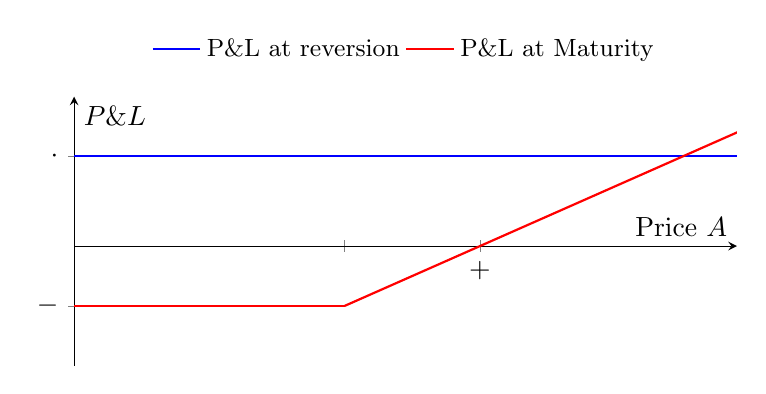
\begin{tikzpicture}[
      declare function={
        mypl(\x)= -1.25 + (\x>25) * (0.9*(\x-25));
      }
    ]
    \begin{axis}[
      xlabel={Price $A$},
      ylabel={$P\&L$},
      axis lines=middle,
      width=10cm,height=5cm,
      xmin=0,xmax=4.9,
      ymin=-2,ymax=2.5,
      ytick={-1,1.5}, 
      xtick={2, 3},
      xticklabels={$\strikePriceShort$, $\strikePriceShort+\premiumShort$},
      yticklabels={$-\premiumShort$, $\premiumShort \cdot \factorPrimitive$},
      legend style={
        draw=none,
        legend columns=-1,
        at={(0.5,1)},
        anchor=south,
        outer sep=1em,
        node font=\small,
      },
    ]
    
      %\addplot[blue,thick] {mypl(x)};
      \addplot[blue,thick] coordinates {(0,1.5) (5,1.5)};
      \addlegendentry{P\&L at reversion}
      %\addplot[pink, thick] {0.05*(x-20)^2-1.25};
      \addplot[red,thick] coordinates {(0,-1) (2,-1)};
      \addplot[red,thick] coordinates {(2,-1) (5,2)};
      \addlegendentry{P\&L at Maturity};
    \end{axis}
    \end{tikzpicture}
    \caption{Payoff \& Loss (P\&L) analysis for the Buyer $\buyerShort$ of the \financialPrimitive. In case of reversion, the payoff for the $\buyerShort$ is constant. In case of maturity, the payoff is equal to a traditional call option.}
    \label{figure:payoffCurve}
\end{figure}

\noindent \textbf{Payoff analysis.}
The buyer $\buyerShort$ is the entity which is entitled to execute the option contract at maturity.
We assume that $\buyerShort$ always acts rationally, such that their financial benefit is maximized. 
In the case of a \financialPrimitive, the payoff which $\buyerShort$ receives can be categorized into two cases~---~\emph{(i)} $\sellerShort$ terminates the option at pre-maturity or \emph{(ii)} the contract is not terminated until maturity at time $\terminationTime$.
In the first case, the payoff for $\buyerShort$ is constant, as the seller $\sellerShort$ reimburses the buyer $\buyerShort$ with $\premiumShort \cdot \factorPrimitive$, where $\factorPrimitive > 1$. 
If the seller $\sellerShort$ does not terminate the contract, the payoff for $\buyerShort$ is equivalent to
\begin{equation}
    P_{\buyerShort} = 
    \begin{cases}
      A(T)-K-\premiumShort & \text{if~} A(T) \geq K \\
      -\premiumShort & \text{if~} A(T) < K
    \end{cases}
\end{equation}
Note, that the payoff in this case is equivalent to a traditional European style call option.
The visualized payoff curves for $\buyerShort$ are presented in Figure~\ref{figure:payoffCurve}.

% High-level payoff analysis as described here https://bookdown.org/maxime_debellefroid/MyBook/a-deeper-understanding-of-options.html#european-call-options

\subsection{The \protocol Protocol}

We present the \protocol protocol in the following. On a high-level, \protocol seeks to mitigate liquidations through \supporters that top-up the collateral of an unhealthy borrowing position (i.e., the health factor declined below one). 
\protocol allows any external entity to become such a \supporter.
We start with an overview of \protocol by outlining the equivalence to \financialPrimitives.
%{\color{red}Successively, we determine the premium that $\supporterShort$ has to pay at initiation to the \borrower $\borrowerShort$, analyze incentives for $\supporterShort$ to engage in \protocol, and highlight considerations for practical instantiations.}

\subsubsection{Overview}

\begin{figure}[tb!]
    \centering
    \includegraphics[width=\columnwidth]{figures/01_Overview.pdf}
    \caption{High-level overview of the \protocol protocol which realizes a reversible call option in \DeFi.
    Once the borrowing position opened by the \borrower $\borrowerShort$ is unhealthy, yet not liquidated, the \supporter $\supporterShort$ is able to top up the collateral in position $\borrowingPositionShort{}$.}
    %Once a borrowing position is tollable, a toller can initiate \protocol. The tolling then terminates either if \emph{(i)} the debt is under-collateralized, \emph{(ii)} the borrower adds collateral, \emph{(iii)} the borrower repays the debt, \emph{(iv)} the collateral price rises, or \emph{(v)} \protocol reaches a full acquisition.}
    \label{fig:high-level-toll}
\end{figure}

% Assumption plain model: HF<1 -> Supporter can engage, we defer liquidations for now and assume that each position is supported sufficiently.

An overview of \protocol is presented in Figure~\ref{fig:high-level-toll}.
On a high-level, \protocol is separated into three phases~---~\emph{(i)} Initialization, \emph{(ii)} pre-Maturity, and \emph{(iii)} Maturity.
We first assume that \protocol replaces the liquidation mechanism in our exemplary lending/borrowing protocol. We defer practical considerations for co-existence of \protocol and liquidations to Section~\ref{subsection:practicalInstantiation}.

\begin{description}[style=unboxed, leftmargin=0cm]
    \item[1) Initialization.]
    We assume the existence of an on-chain \lendingPool $\lendingPoolShort$ with a single borrowing position $\borrowingPositionShort{} = \langle \numberCoinsDebt{t}, \numberCoinsCollateral{t} \rangle$ initialized by the \borrower $\borrowerShort$.
    The supporter can engage at time $\initiateTime$, if the following condition holds:
    
    \begin{equation}
    \label{equation:HF}
    \healthFactorShortTwo{\initiateTime}{\borrowingPositionShort{}} = 
    \frac{\numberCoinsCollateral{\initiateTime} \cdot \priceInp{\initiateTime} \cdot \collateralDiscountShort}{\numberCoinsDebt{\initiateTime}} < 1
    \end{equation}

%     \begin{equation}\collateralizationRatioShort{\borrowingPositionShort{}}=\frac{\numberCoinsCollateral{t} \cdot \price}{\numberCoinsDebt{t}}>1
% \end{equation}

In words, the \healthFactor should be lower than one. Note that the position may be over-collateralized ($\collateralizationRatioShortTwo{\initiateTime}{\borrowingPositionShort{}} > 1$) or under-collateralized  ($\collateralizationRatioShortTwo{\initiateTime}{\borrowingPositionShort{}} < 1$), depending on the steepness of the price decline that yields a \borrowingPosition unhealthy.
%, whereas the \collateralizationRatio is still greater than one such that the position is still overcollateralized.
At this point, $\supporterShort$ buys a \financialPrimitive by topping-up $\factorMiqado \cdot \numberCoinsCollateral{\initiateTime}$ into $\borrowingPositionShort{}$, which grants the right to take over the \borrowingPosition $\borrowingPositionShort{}$ at maturity $\terminationTime$.
The price of the \financialPrimitive hence is $\factorMiqado \cdot \numberCoinsCollateral{\initiateTime}$. Note that the premium factor $\factorMiqado$ is a protocol parameter that can be ruled in the lending pool contract. To decide whether to deposit, a supporter would need to price the \financialPrimitive and estimate its potential profitability, which we detail in Section~\ref{sec:pricing}.%, which is a mutliple of the collateral deposited by $\borrowerShort$ when initializing $\borrowingPositionShort{}$. %The factor $\factorMiqado$ is chosen such that the health factor 
% \begin{equation}
%     \healthFactorShortTwo{\initiateTime+1}{\borrowingPositionShort{}} = 
%     \frac{(1+\factorMiqado) \cdot \numberCoinsCollateral{\initiateTime} \cdot \price \cdot \collateralDiscountShort}{\numberCoinsDebt{\initiateTime}} > \healthFactorShortTwo{\initiateTime}{\borrowingPositionShort{}}
% \end{equation}
% is greater than the previous health factor, hence the borrowing position is returned to a healthy state and cannot face liquidation. Note, that this is equivalent to pricing a \financialPrimitive.
% We elaborate on the pricing model in Appendix~\ref{app:pricing}.


\item[2) pre-Maturity.]
Once $\supporterShort$ acquires a \protocol option with maturity $\terminationTime$, the pre-maturity stage starts.
At any point $\initiateTime < \Time < \terminationTime$, the borrower $\borrowerShort$ can terminate the \protocol protocol by repaying $\supporterShort$ the premium $\factorMiqado \cdot \numberCoinsCollateral{\initiateTime}$ multiplied by a constant factor $\factorMiqadoRe$ that incentivizes the initial support of $\supporterShort$, hence 

\begin{equation}
    \returnPaymentShort = \factorMiqado \cdot \numberCoinsCollateral{\initiateTime} \cdot (1+\borrowingInterestRate) \cdot \factorMiqadoRe 
\end{equation}

where $0 < \borrowingInterestRate < 1$ is the interest rate which $\borrowerShort$ agreed to pay for its loan when initiating the position $\borrowingPositionShort{}$.
The factor $0 < \factorMiqadoRe < 1$ is implementation dependent and should account for the risk $\supporterShort$ has to take when supporting a position.
%a variable agreed upon between $\borrowerShort$ and $\supporterShort$ 
    
\item[3) Maturity.]
At Maturity, there are two possible options how the \protocol protocol may terminate. The payoff for the \supporter $\supporterShort$ in the case of maturity is depicted in Figure~\ref{figure:payoffCurve}.
\begin{enumerate}
    \item \textbf{Full Takeover.}
    % Full Takeover when price is smaller than Strike price + factorMiqdo * C_0 ->
    In general, \protocol option contracts have an ``Out-of-the-Money'' strike price $\strikePriceShort$, such that the strike is greater than the collateralization ratio upon initiation of the position $\borrowingPositionShort{}$ by $\borrowerShort$. Essentially, as the health factor is lower than one, the intrinsic value of the option is low, whereas the time value based on volatility and time of expiration is high.
    %As a result, $\supporterShort$ only takes over the full position if the health factor of the position at maturity is greater than at initiation, such that 
    % T > t_0  
% $\healthFactorShortTwo{\terminationTime}{\borrowingPositionShort{}} > \healthFactorShortTwo{\initiateTime}{\borrowingPositionShort{}}$.
    % If the price of the  is $>\strikePriceShort$
    %\item \textbf{Payback.}
    % Supporter
    %For payback, the price increase is smaller than 

    \item \textbf{Default.}
    The \supporter defaults and does not exercise the option, hence loses the premium $\premiumShort$ (cf. Figure~\ref{figure:payoffCurve}), if the price at Maturity is below the strike price $\strikePriceShort$. In this case, where \protocol fully replaces the liquidation mechanism, another round of Miqado initiates. Rational \supporters initiate a \protocol session if the condition presented in \emph{1.) Initialization} is fulfilled.
    
\end{enumerate}
% Two options for the supporter - take over the full position, do not take over the full position
% This is only rational, if 1) the health factor is significantly over 1, 2) the position is still over-collateralized.
% If the position is at this point under-collateralized, we face the situation that 
    
\end{description}

% \begin{table}[t]
%     \centering
%     \caption{Caption}
%     \begin{tabular}{c|c}
%     \toprule
%          &  \\
%     \midrule
%          & \\
%     \bottomrule
%     \end{tabular}
%     \label{tab:my_label}
% \end{table}

\subsubsection{Incentive Discussion}
% As described in previous analysis, based on Black-Scholes
% Why would the supporter engage in this?
% Why would the supporter engage in the MIQADO protocol?

A common question is why a \supporter would actually engage in the \protocol protocol and top up liquidity positions that are unhealthy.
In general, whether a \supporter is incentivized to engage in a \protocol option in a \FSL liquidity pool depends on the price volatility and the selected strike price.
Given the volatility of various cryptocurrencies, it is infeasible to draw a general conclusion fitting all scenarios.
\Supporters can price the \protocol options and compare to the required cost (i.e., the premium) to evaluate the potential risks. We outline a pricing model for \financialPrimitives in Section~\ref{sec:pricing}.
%evaluate whether a, as $\factorMiqado$ is an indicator for the risk a \supporter wants to take.
In practice, we assume that \supporters taking a low risk will face termination at pre-maturity by $\borrowerShort$, yielding a smaller payoff for $\supporterShort$.
We empirically evaluate \protocol's ability to prevent \liquidationSpirals by replacing the liquidation mechanism in Section~\ref{sec:empirical}.

%In general, the \supporter is incentivized to participate, if the cost of initiating a \protocol option is lower than initiat
% \begin{equation}
%     c_{\protocol} = \factorMiqado \cdot \numberCoinsCollateral{\initiateTime} \cdot \priceInp{\initiateTime} < c_{BS-model}
% \end{equation}

%%% High level overview of protocol idea

% Initialization: 
%   Borrower creates position
%   Price decline, HF<1, still over-collateralized!
%   Borrower allows for top-up, Supporter engages by topping up the position with lambda * C

% pre-Maturity:
%   Borrower is allows to terminate the protocol, paying back lambda * C + EXTRA to the supporter

% Maturity:
% 

%%% Analogy - reversible call option

% Assumption: If the supporter decides to buy, he buys the whole position and not a partial stake in the position!
% Benefit: No naked selling of call options possible. The seller of the call option always has the underlying assets. -> Less systemic risk

\subsection{Pricing \FinancialPrimitive}\label{sec:pricing}
The \financialPrimitive is equivalent to an European call option in the case of maturity. Therefore, we can apply the widely adopted Black-Scholes pricing model~\cite{hull2003options} for European call options to \protocol.
We outline the B-S model details in Appendix~\ref{app:bs-model}.
We assume that at initialization $\initiateTime$, the \supporter $\supporterShort$ buys a \protocol option by supplying $\factorMiqado \cdot \numberCoinsCollateral{\initiateTime}$ of additional collateral priced at $\factorMiqado \cdot \numberCoinsCollateral{\initiateTime} \cdot \priceInp{\initiateTime}$.
    The spot exchange rate is equivalent to $\priceInp{\initiateTime}$, whereas the domestic interest rate $\domesticInterestRate$ is equivalent to the borrowing interest rate of the protocol $\borrowingInterestRate$.
    The foreign interest rate $\foreignInterestRate$ remains the same.
    The volatility $\volatilityAsset$ can be calculated from the price history.
    Henceforth, the optimal factor $\factorMiqado^{*}$ following the B-S model can be calculated as%which determines the amount of collateral $\supporterShort$ has to supply can be calculated as 
    \begin{equation}
    \label{equation:price}
        \factorMiqado^{*} = \frac{\priceInp{\initiateTime} e^{-\foreignInterestRate \cdot \terminationTime} N(d_1) - \strikePriceShort e^{-\borrowingInterestRate \cdot \terminationTime} N(d_2)}{\numberCoinsCollateral{\initiateTime} \cdot \priceInp{\initiateTime}}
    \end{equation}
    with equations for $d_1$ and $d_2$ outlined in Appendix~\ref{app:bs-model}. A \supporter then compares the actual premium factor $\factorMiqado$ set by the lending protocol to $\factorMiqado^{*}$ and evaluates the profitability. In practice, a supporter would have a personalized pricing model based on the supporter's predictions on the price dynamics and risk preference.
    
    % We defer pricing models for \financialPrimitives that take into account the decrease in risk and lowered average payoff due to termination by $\sellerShort$, to future works.

\subsection{Practical Instantiation}
\label{subsection:practicalInstantiation}

\begin{figure}[tb!]
    \centering
    \includegraphics[width=0.75\columnwidth]{figures/02_Race.pdf}
    \caption{
    Practical Instantiation of \protocol on top of a traditional liquidation mechanism.
    The \supporter $\supporterShort$ has an advantage over the liquidator $\liquidatorShort$ to support a temporarily unhealthy position.
    }
    % High-level overview of the \protocol protocol which realizes a reversible call option in \DeFi.
    % Once the borrowing position opened by the \borrower $\borrowerShort$ is unhealthy, yet not liquidated, the \supporter $\supporterShort$ is able to top up the collateral in position $\borrowingPositionShort{}$.}
    %Once a borrowing position is tollable, a toller can initiate \protocol. The tolling then terminates either if \emph{(i)} the debt is under-collateralized, \emph{(ii)} the borrower adds collateral, \emph{(iii)} the borrower repays the debt, \emph{(iv)} the collateral price rises, or \emph{(v)} \protocol reaches a full acquisition.}
    \label{fig:practical-instantiation}
\end{figure}


% SF = CR * (collateral discount + Buffer), HF = CR * collateral discount, Buffer > 0
When there is no \supporter $\supporterShort$ willing to purchase a \financialPrimitive or when a \supporter defaults, the \lender $\lenderShort$ faces a loss as the \borrower  $\borrowerShort$ is not incentivized to repay the outstanding debt and $\supporterShort$ is not incentivized to take over the position $\borrowingPositionShort{}$.
In a practical instantiation (cf.\ Figure~\ref{fig:practical-instantiation}), a protocol operator may want to operate \protocol options on top of a traditional liquidation mechanism in order to prevent this.
As such, the protocol can employ a buffer to derive an additional \textit{support factor} $\supportFactorShort$, such that $\supporterShort$ can engage in a \protocol option if 
\begin{equation}
    \supportFactorShort = \collateralizationRatioShortTwo{\initiateTime}{\borrowingPositionShort{}} \cdot (\collateralDiscountShort + \bufferShort) < 1
\end{equation}
where $\bufferShort$ is the buffer parameter, s.t.\ $\bufferShort > 1$.

A liquidator can additionally engage when the health factor is lower than one, as traditionally assumed and presented in Equation~\ref{equation:HF}.
With this construction, the \supporter has an advantage over the \liquidator to support a temporarily unhealthy position and make a profit.
Effectively, this construction similarly mitigates \liquidationSpirals, dependent on the buffer $\bufferShort$.

\subsection{Remarks}
\protocol enhances Fixed Spread Liquidations in the following aspects:
\begin{description}[style=unboxed, leftmargin=0cm]
    \item[Rescue Opportunity.] The reversible call option of \protocol offers a time window for a borrower to rescue its borrowing position. With a fixed spread liquidation, the close factor is usually larger than necessary such that more collateral is sold off at a discount, which negatively impacts the borrowers financial interests. With \protocol options, this risk is alleviated, such that over-liquidation is not a concern and the \borrower has to pay less to rescue its position.
    \item[Collateral Restraint.] \protocol absorbs additional collateral and locks it in the lending pool until the reversible call option's maturity. This mitigates the possible \liquidationSpiral, which we quantitatively show in Section~\ref{sec:empirical}.
    \item[\MEV Mitigation.] \FSL liquidations provides deterministic and cost-free  opportunities for miners to profit through manipulating transaction order and front-running other liquidators. In \protocol, if a miner deems a reversible call option profitable, it still has an advantage over other supporters. This is because a miner can single-handedly front-run any competing transaction and be the first to initiate \protocol. Nevertheless, as shown in Section~\ref{sec:protocol-evaluation}, a \protocol reversible call option does not guarantee a profit. Moreover, a supporter bears a capital cost while locking the premium in the lending pool. We hence conclude that \protocol mitigates the \MEV problem.
    %\item[Health Factor Improvement]
\end{description}

\section{Empirical Evaluation}\label{sec:empirical}
In this section, we evaluate the \protocol protocol by comparing \protocol to the dominant liquidation mechanism \FSL. To this end, we collect all liquidation events on Aave (both V$1$ and V$2$) and Compound from the~\StartDate to the~\EndDate. Aave and Compound are the top two lending protocols on Ethereum in terms of \TVL, according to \href{https://defillama.com/protocols/lending/Ethereum}{defillama.com}. Both of the two lending protocols follow the \FSL mechanism (cf.\ Section~\ref{sec:fixed-spread-liquidation}). In total, we collect~\TotalLiquidationEvents liquidations (Aave V1:~\AaveVOneLiquidations; Aave V2:~\AaveVTwoLiquidations; Compound:~\CompoundLiquidations). %In the following, we first quantify the downward price spiral caused by \FSL and then simulate how \protocol could have performed in these liquidation events.

\subsection{Quantifying \LiquidationSpiral}\label{sec:quantifying}
% We start with quantifying the downward price spiral deteriorated by \FSL.
\subsubsection{Collateral Release.}

A lending protocol that applies \FSL directly sells the liquidated collateral to the \liquidator at a discount. 
This aggravates the price downtrend of the liquidated cryptocurrency as \liquidators may immediately sell of the acquired collateral, which was locked in the lending protocol, to secondary markets.
%\FSL aggravates the price downtrend of a liquidated cryptocurrency, because the \FSL mechanism directly releases the liquidated collateral, which was locked in the lending protocol, to the markets. 
Precisely measuring the impact of \FSL on the liquidated collateral price is challenging. We need to devise an accurate economic model to exclude the impact of other factors, such as the demand change for the collateral. We also need to model the liquidity dynamics on various centralized and decentralized exchanges at the time of liquidation. These challenges are however beyond the scope of this study and are left for future work. Therefore, we choose to present the value of collateral that is released in the \FSL liquidations (cf.\ Metric~\ref{metric:release}) to intuitively quantify the \liquidationSpiral introduced by the \FSL mechanism.

\newtheorem{metric}{Metric}
\begin{metric}[\FSL Collateral Release]\label{metric:release}
The value of collateral released to the markets in a \FSL liquidation.
\end{metric} 
Figure~\ref{fig:collateral_release} presents the monthly collateral release in the past~\TotalLiquidationEvents \FSL liquidations. The total collateral release amounts to~\LiquidatedCollateral over the~\liquidationTimeFrame.

\begin{figure}[t]
    \centering
    \includegraphics[width=\columnwidth]{figures/collateral_release_restraint.pdf}
    \caption{Over a time-frame of~\liquidationTimeFrame (from the~\StartDate to the~\EndDate), the collateral release by the \FSL mechanism accumulates to~\LiquidatedCollateral, with a monthly peak of~\CollateralReleasePeak in May,~$2021$. On the contrary, our \protocol protocol restrains additional collateral in the lending pool instead of releasing and further mitigates the \liquidationSpiral. The accumulative collateral restraint by \protocol (cf.\ Metric~\ref{metric:restraint}, Section~\ref{sec:protocol-evaluation}) amounts to~\CollateralRestraintTwenty~USD when the premium factor $\lambda$ is set to~$20\%$.}
    \label{fig:collateral_release}
\end{figure}

\subsubsection{Direct Price Decline.}
In Case Study~\ref{casestudy:deleveraging-spiral} (cf.\ Section~\ref{sec:motivation}), we show that a liquidator can choose to sell the collateral acquired from the borrower within the liquidation transaction. We observe that such a ``sell-after-liquidation'' strategy is prevalent, which we define as a short liquidation (cf.\ Definition~\ref{def:short-liquidation}). 
\begin{definition}[Short Liquidation]\label{def:short-liquidation}
In a short liquidation, $\liquidatorShort$ sells (fully or partially) the collateral acquired from $\borrowerShort$ within the liquidation transaction.
\end{definition}
To identify a short liquidation, we first gather the ERC-20 transfer and asset swap events from a liquidation transaction.\footnote{ERC-20 is a fungible token standard, which is extensively adopted in the Ethereum \DeFi ecosystem. An event refers to a log emitted by a smart contract during its execution. These events are identifiable by a unique topic hash and can represent various actions, such as an asset swap on a decentralized exchange. In this work, for asset swap events, we captured the most liquid exchanges on Ethereum including Uniswap V1, V2, V3, Sushiswap, and Curve.} With these events, we then filter the exchange contracts that are potentially used for collateral selling. The filtering process is based on two criteria: \textit{(i)} the contract emits an asset swap event during the transaction execution; \textit{(ii)} the contract receives the liquidated collateral token (fully or partially). If such an exchange contract is detected, the liquidation transaction is classified as a short liquidation.
From the~\TotalLiquidationEvents studied liquidations, we identify~\ShortLiquidations short liquidations. In total,~\ShortLiquidationUSDSold of collateral is sold directly by the liquidators in these short liquidations. We find that in~\FullySoldShortLiquidations of the short liquidations, the acquired collateral is fully sold. On average,~\ShortLiquidationsSellPercentageAverage of the collateral is sold in a short liquidation.

A short liquidation directly leads to a collateral price decline on the exchange where the liquidator sells the acquired collateral. Although a significant price change in a single market will eventually be evened out by arbitrageurs\footnote{Entities who profit by leveraging price differences across different markets.} among all available markets, while the negative impact on the collateral price remains. We therefore apply such a price decline as a metric of how \FSL liquidations destabilize lending protocols (cf.\ Metric~\ref{metric:price-decline}).

\begin{metric}[Direct Price Decline]\label{metric:price-decline}
In a short liquidation, the spot price decline on the exchange where the liquidator sells the acquired collateral.
\end{metric}
We find that the average collateral price decline led by the~\ShortLiquidations short liquidations is~\ShortLiquidationPriceDeclineAverage, while the maximal decline reaches~\ShortLiquidationPriceDeclineMax.\footnote{Cf.\ \etherscantx{0xff2d484638b846a46b203a22b02d71df44bf78346c72b954ad0ad05f34b134c8}}

\subsection{\protocol Evaluation}\label{sec:protocol-evaluation}
In the following, we assume that Aave and Compound had adopted \protocol and simulate how \protocol could have outpaced \FSL in the past liquidation events. Our simulation is constrained to every single liquidation event, while ignoring the long-term impact of \protocol. For example, \protocol mitigates the price downtrend and hence could have prevented follow-up liquidations in a \liquidationSpiral, which we leave for future research.

The performance of \protocol is influenced by its parameters. In our simulation, we assume that \protocol follows the corresponding lending protocol's configuration for the collateral discount $\collateralDiscountShort$ at the time of each liquidation. This implies that \protocol shares the same triggering condition as \FSL (i.e., when the health factor declines below one) and hence applies to every liquidated borrowing position. We also need to parameterize the premium factor $\lambda$ and the time to maturity $\Delta T$ for the reversible call option. Similar to how the parameters for lending protocols evolve,\footnote{\url{https://docs.aave.com/risk/asset-risk/risk-parameters}.} these two parameters need to be empirically determined and dynamically adjusted given various market conditions (e.g., the price volatility). We therefore simulate on various specific settings to show how \protocol performs under different configurations.

\subsubsection{Collateral Restraint.} \protocol absorbs additional collateral, which is restrained in the lending pool during the protocol execution. This collateral restraint, contrary to \FSL's supply release (cf.\ Metric~\ref{metric:release}), imposes a positive impact on stabilizing collateral price (cf.\ Metric~\ref{metric:restraint}).
\begin{metric}[\protocol Collateral Restraint]\label{metric:restraint}
The value of collateral deposited by the \supporter in a \protocol execution.
\end{metric}
We visualize the monthly comparison between the collateral restraint by \protocol and the collateral release by \FSL in Figure~\ref{fig:collateral_release}. The accumulative collateral restraint with different parameters is outlined in Table~\ref{tab:accumulative_collateral_restraint}, Appendix~\ref{app:tables}. We find that when $\lambda$ is~$20\%$, the accumulative collateral restraint reaches~\CollateralRestraintTwenty~USD. Notably, as a by-product, the restrained additional collateral is counted towards the lending pool's \TVL, which is a common protocol success metric.

\subsubsection{Health Factor Recovery.} One shared target of \protocol and \FSL is to increase the health factor of a borrowing position. In Figure~\ref{fig:health_factor_distributions}, we present the health factor distributions before and after the studied \FSL liquidations. We further simulate how \protocol could have increased the health factor with different parameters. We find that,~\HealthyPositionsAfterFSL of the liquidated positions become healthy (the health factor is increased above one) after a \FSL liquidation. When $\lambda$ is set to $5\%$, \protocol achieves the same performance (\HealthyPositionsAfterMiqadoLambdaFive~of the borrowing positions become healthy after the supporter deposits). 

\begin{figure}[t]
    \centering
    \includegraphics[width=\columnwidth]{figures/health_factor_distributions.pdf}
    \caption{The health factor distributions pre- and post-\FSL liquidations. We also visualize how \protocol increases the health factor with different premium factors.}
    \label{fig:health_factor_distributions}
\end{figure}

\subsubsection{Payoffs for \Supporter.} We proceed to simulate the payoffs of \protocol supporters. 
In this section, we assume that the borrowers would not terminate the reversible call options. We parameterize $\Delta T$ to $1$, $6$, and $24$ hours and apply the real market price to value every reversible call options at maturity. A supporter then chooses to exercise the option when the value of collateral exceeds the outstanding debt at maturity, and defaults otherwise (cf.\ Figure~\ref{figure:payoffCurve}). In Table~\ref{tab:payoffs}, Appendix~\ref{app:tables}, we outline the probability that a supporter \textit{(i)} exercises the call option and profits, \textit{(ii)}  exercises the call option but loses, \textit{(iii)} defaults, under different parameters. We also present the average profit for every supporter. We show that, to our surprise, the \protocol premium factor does not impact the probability of the reversible call option in practice. Notably, in Table~\ref{tab:payoffs}, we assume that the borrowers would not rescue their debts and therefore conjecture that the actual payoffs for supporters would be lower than the presented results.


\subsubsection{Collateral Release Reduction} In practice, the probability that a \protocol supporter may default on the reversible call option is up to~$13.48\%$. This implies that the associated borrowing position is under-collateralized at maturity and may be further available for \FSL (cf.\ Section~\ref{subsection:practicalInstantiation}). We simulate that, in the worst case, the collateral release by \FSL after \protocol (cf.\ Metric~\ref{metric:release}) amounts to~\CollateralReleaseWithMiqado, which is a reduction of~\CollateralReduction compared the~\LiquidatedCollateral collateral release by \FSL only (cf.\ Section~\ref{sec:quantifying}).

 

\section{Related Work}\label{sec:related-work}
%here is a growing body of literature studying \DeFi. 
Various works in \DeFi focus on lending \& borrowing protocols from diverse perspectives such as economics, security and formal modeling.
Kao \etal~\cite{kao2020analysis} evaluate the economic security of Compound by using agent-based simulation. Darlin \etal~\cite{darlin2020optimal} investigate the optimal bidding strategies for auction liquidations. Perez \etal~\cite{perez2021liquidations} present an empirical analysis of liquidations on Compound. Qin \etal~\cite{qin2021empirical} perform a longitudinal study on the liquidation events of four major Ethereum lending pools (i.e., Aave, Compound, dYdX, and MakerDAO), while showing the over-liquidation problem of the fixed spread liquidations. In this work, we show that the proposed \protocol protocol mitigates these problems. Bartoletti~\etal systematize \DeFi lending pools~\cite{bartoletti2021sok} and further provide a formal analysis of \DeFi lending pools~\cite{bartoletti2022formal}. Wang \etal~\cite{wang2022speculative} study under-collateralized \DeFi lending platforms showing the three main risks of a leverage-engaging borrower, namely, impermanent loss, arbitrage loss, and collateral liquidation. Select stablecoin designs leverage lending and borrowing mechanisms (e.g., DAI from MakerDAO), as studied in~\cite{klages2022while,klages2020stablecoins,klages2019stability}.

Besides \DeFi lending and borrowing, further studies focus on decentralized exchanges and the security of the \DeFi ecosystem~\cite{daian2020flash,zhou2021high,qin2021attacking,qin2022quantifying,zhou2022sok}. 
Most recently, Zhou~\etal~\cite{zhou2022sok} systematize attacks on \DeFi and highlight the need for further research on the protocol layer due to $59$\% of attacks on lending \& borrowing platforms yielding from insufficient protocol design. 
%Cryptocurrency liquidations in centralized exchanges are studied in~\cite{soska2021towards}.

Further, there are various non-academic works that offer call options in decentralized applications.
\href{https://www.hegic.co/}{Hegic} offers gas-free option trading for ETH and BTC. \href{https://www.ribbon.finance/}{Ribbon} supports on-chain options, where the option price, or premium, is set through an auction. However, none of the existing decentralized applications applies an equivalent financial primitive to lending \& borrowing platforms to mitigate liquidations.


\section{Conclusion}\label{sec:conclusion}

We presented \protocol, the first liquidation mitigation protocol. 
Whereas existing lending and borrowing protocols rely on plain liquidation mechanisms, \protocol secures \borrowingPositions by incentivizing external entities to provide additional collateral.
To facilitate \protocol, we introduce \financialPrimitives, a novel financial primitive with promising properties for application in \protocol.
%\protocol secures collateralized debts by incentivizing external entities to provide additional collateral  instead of selling the provided collateral at a discount in liquidations. 
To highlight the need for \protocol, we show that fixed spread liquidations trigger \liquidationSpirals and destabilize lending markets.
We evaluate \protocol by executing \protocol logic on past blockchain states. We show that by applying \protocol, the amount of liquidated collateral can be reduced by~\CollateralReduction.
By providing a plug-in replacement to existing liquidation mechanisms, \protocol can prevent systemic-failures without extensive overhead.
%, which can be mitigated with \protocol. 
%We analyze the incentive compatibility and risks of \protocol and show how the protocol improves the collateralization status of lending pools. As shown in our empirical evaluation, \protocol could have effectively increased the TVL of lending pools, Aave and Compound, by~\EffectiveTVLIncrease on the~19th of May,~2021~when the cryptocurrency market collapsed by more than $40$\%.

\subsubsection*{Acknowledgements} We thank the anonymous reviewers for the thorough reviews and helpful suggestions that significantly strengthened the paper. This work is partially supported by Lucerne University of Applied Sciences and Arts, the Federal Ministry of Education and Research of Germany (in the programme of ``Souverän. Digital. Vernetzt.''. Joint project 6G-life, project identification number: 16KISK002), and the Algorand Centres of Excellence programme managed by Algorand Foundation.% Any opinions, findings, and conclusions or recommendations expressed in this material are those of the author(s) and do not necessarily reflect the views of Algorand Foundation.

\bibliographystyle{splncs04}
\bibliography{references.bib}

\appendix
% % \newtheorem{lemma}[theorem]{Lemma}
% \section{Lemmas and Proofs}
% \begin{lemma}
% A fixed spread liquidation does not strictly increase the health factor of a borrowing position.
% \end{lemma}
% \begin{proof}

% \end{proof}

% \begin{lemma}
% The collateral deposited by a supporter in \protocol strictly increases the health factor of a borrowing position.
% \end{lemma}
% \begin{proof}

% \end{proof}

\section{Black-Scholes Model}
\label{app:bs-model}
%%% Black-Scholes model to price the call option.
%To determine the premium $\premiumShort = \factorMiqado \cdot \numberCoinsCollateral{\initiateTime}$ paid by a \supporter 
We apply the Black-Scholes model~\cite{black1973pricing} to price call options under optimal assumptions, such as the non-existence of dividend  payouts. %We first introduce the pricing model derived by Black-Scholes and successively derive its application to a \protocol option.
% \begin{description}[style=unboxed, leftmargin=0cm]
% \subsection{Black-Scholes Model}
The option premium is calculated for European call options on a per-share basis. The payoff for $\sellerShort$ introduced in Figure~\ref{figure:payoffCurve} is trivial to grasp but it does not yield any insights on the pricing of the option.
    With the BS model for a European call option determines the option price as
    \begin{equation}
        c = \spotExchangeRate e^{-\foreignInterestRate \cdot \terminationTime} N(d_1) - \strikePriceShort e^{-\domesticInterestRate \cdot \terminationTime} N(d_2)
    \end{equation}
    where
    \begin{equation}
        d_1 = \frac{\ln(\spotExchangeRate\/\strikePriceShort)+(\domesticInterestRate-\foreignInterestRate+\volatilityAsset^2\/2) \cdot \terminationTime}{\volatilityAsset\cdot \sqrt{\terminationTime}}
    \end{equation}
    and 
    \begin{equation}
        d_2 = d_1 - \volatilityAsset\cdot \sqrt{\terminationTime}.
    \end{equation}
    $\spotExchangeRate$ is the spot exchange rate, $\foreignInterestRate$ is the foreign interest rate, $\domesticInterestRate$ is the domestic interest rate and $\volatilityAsset$ is the volatility of the underlying asset.
    For a detailed introduction to the Black-Scholes pricing model for European call options, we refer the interested reader to~\cite{hull2003options}.
    
We remark that the B-S model does not take into account the decrease in risk and lowered average payoff due to termination by $\sellerShort$. We defer a more precise pricing model for \financialPrimitives that to future work.

% \subsection{Application to \protocol}
%     To apply the BS-model to \protocol, we assume that at initialization $\initiateTime$, the \supporter $\supporterShort$ buys a \protocol option by supplying $\factorMiqado \cdot \numberCoinsCollateral{\initiateTime}$ of additional collateral priced at $\factorMiqado \cdot \numberCoinsCollateral{\initiateTime} \cdot \priceInp{\initiateTime}$.
%     The spot exchange rate is equivalent to $\priceInp{\initiateTime}$, whereas the domestic interest rate $\domesticInterestRate$ is equivalent to the borrowing interest rate of the protocol $\borrowingInterestRate$.
%     The foreign interest rate $\foreignInterestRate$ remains the same.
%     The volatility $\volatilityAsset$ can be calculated from the slope of the price decline that drove $\borrowingPositionShort{}$ into an unhealthy state.
%     Henceforth, the factor $\factorMiqado$ which determines the amount of collateral $\supporterShort$ has to supply can be calculated as 
%     \begin{equation}
%     \label{equation:price}
%         \factorMiqado = \frac{\priceInp{\initiateTime} e^{-\foreignInterestRate \cdot \terminationTime} N(d_1) - \strikePriceShort e^{-\borrowingInterestRate \cdot \terminationTime} N(d_2)}{\numberCoinsCollateral{\initiateTime} \cdot \priceInp{\initiateTime}}
%     \end{equation}
%     with equations for $d_1$ and $d_2$ following the same reasoning as above. We defer pricing models for \financialPrimitives that take into account the decrease in risk and lowered average payoff due to termination by $\sellerShort$, to future works.
\clearpage
\section{Tables}\label{app:tables}

\begin{table}[]
    \centering
    \caption{Accumulative collateral restraint by \protocol over a time-frame of~\liquidationTimeFrame.}
    \begin{tabular}{cc|cccccccccc}
    \toprule
    \protocol Premium Factor $\lambda$ &&& $1\%$ && $2\%$ && $5\%$ && $10\%$ && $20\%$ \\\midrule
     Accumulative Collateral Restraint (USD) &&& \CollateralRestraintOne && \CollateralRestraintTwo && \CollateralRestraintFive && \CollateralRestraintTen && \CollateralRestraintTwenty\\
    \bottomrule
    \end{tabular}
    \label{tab:accumulative_collateral_restraint}
\end{table}

\begin{table}[]
\centering
\caption{Payoffs for \protocol supporters at maturity assuming that borrowers would not rescue. We present the probability that a supporter \textit{(i)} exercises the call option and profits, \textit{(ii)}  exercises the call option but loses, \textit{(iii)} defaults. We also simulate the average profit for supporters. our simulations are based on the real market prices.}
\resizebox{\columnwidth}{!}{%
\begin{tabular}{c|ccccc|c}
\toprule
           $\lambda$           & $1\%$ & $2\%$ & $5\%$ & $10\%$ & $20\%$                  &     $\Delta T$                      \\ \midrule
\multicolumn{1}{c|}{$+$} & $87.46\%$    &   $87.46\%$  &   $87.46\%$  &   $87.46\%$   & \multicolumn{1}{c|}{$87.46\%$} & \multirow{4}{*}{1hour}    \\
\multicolumn{1}{c|}{$-$} & $0.29\%$    &  $0.58\%$   &  $1.41\%$   &  $2.47\%$    & \multicolumn{1}{c|}{$4.14\%$} &                           \\
\multicolumn{1}{c|}{$\#$} & $12.25\%$   &  $11.96\%$   &  $11.13\%$   &  $10.08\%$    & \multicolumn{1}{c|}{$8.41\%$} &                           \\
\multicolumn{1}{c|}{$\$$} &  $125.51$K$\pm1.52$M   &  $125.51$K$\pm1.52$M    &  $125.50$K$\pm1.52$M    &  $125.49$K$\pm1.52$M     & \multicolumn{1}{c|}{$125.48$K$\pm1.52$M} &                           \\\midrule
\multicolumn{1}{c|}{$+$} & $87.19\%$    &  $87.19\%$   &  $87.19\%$   &   $87.19\%$   & \multicolumn{1}{c|}{$87.19\%$} & \multirow{4}{*}{6 hours}  \\
\multicolumn{1}{c|}{$-$} &  $0.30\%$   &   $0.60\%$  &   $1.50\%$  &  $2.68\%$    & \multicolumn{1}{c|}{$4.44\%$} &                           \\
\multicolumn{1}{c|}{$\#$} &  $12.51\%$   &   $12.21\%$  &  $11.31\%$   &  $10.13\%$    & \multicolumn{1}{c|}{$8.37\%$} &                           \\
\multicolumn{1}{c|}{$\$$} &  $154.01$K$\pm2.19$M   &  $154.01$K$\pm2.19$M   &  $154.00$K$\pm2.19$M   &  $154.00$K$\pm2.19$M    & \multicolumn{1}{c|}{$154.98$K$\pm2.19$M} &                           \\\midrule
\multicolumn{1}{c|}{$+$} & $85.95\%$    &  $85.95\%$   &   $85.95\%$  &  $85.95\%$    & \multicolumn{1}{c|}{$85.95\%$} & \multirow{4}{*}{24 hours} \\
\multicolumn{1}{c|}{$-$} &  $0.56\%$   &  $1.03\%$   &  $2.16\%$   &   $3.62\%$   & \multicolumn{1}{c|}{$5.59\%$} &                           \\
\multicolumn{1}{c|}{$\#$} &  $13.48\%$   &  $13.02\%$   &  $11.89\%$   &  $10.42\%$    & \multicolumn{1}{c|}{$8.45\%$} &                           \\
\multicolumn{1}{c|}{$\$$} & $144.42$K$\pm1.83$M    &  $144.40$K$\pm1.83$M   &   $144.36$K$\pm1.83$M  &   $144.32$K$\pm1.83$M   & \multicolumn{1}{c|}{$144.29$K$\pm1.83$M} &                           \\\bottomrule
\end{tabular}%
}
\begin{tabular}{lllll}
$+$ exercise and profit &\qquad\qquad& $-$ exercise but lose &\qquad\qquad& $\#$ default\\
\multicolumn{5}{l}{$\$$ average profit for supporters in USD (mean$\pm$std)}
\end{tabular}
\label{tab:payoffs}
\end{table}

\end{document}
